用前面的例子来了解移动语义是如何实现的。

实现移动语义之前,\textit{std::vector<>}只有一个\textit{push_back()}的实现(这里简化了vector的声明):

\begin{cppcode}
template<typename T>
class vector {
	public:
	...
	// insert a copy of elem:
	void push_back (const T& elem);
	...
};
\end{cppcode}

传递参数给\textit{push_back()}的方法只有一种:将其绑定到\textit{const}引用上。\textit{push_back()}的实现方式是在不修改参数的情况下,创建参数的副本。

C++11开始,\textit{push_back()}有了重载:

\begin{cppcode}
template<typename T>
class vector {
	public:
	...
	// insert a copy of elem:
	void push_back (const T& elem);
	// insert elem when the value of elem is no longer needed:
	void push_back (T&& elem);
	...
};
\end{cppcode}

第二个\textit{push_back()}使用了为移动语义引入的新语法。使用两个\&声明实参,不使用\textit{const},这样的参数称为\begin{cppcode}
右值引用}}。只有一个\&的“普通引用”现在称为\textit{\textbf{左值引用
\end{cppcode}。在这两个调用中,都传递了通过引用插入的值。但是,区别如下:

\begin{itemize}
	\item 使用\textit{push_back(const T\&)},可以保证不修改传递的值。

	当调用者仍然需要传递的值时,将调用此函数。
	\item 通过\textit{push_back(T\&\&)},可以修改传递的实参(因此它不是\textit{const})来“窃取”值。语义上的含义是,新元素接收传递的值,但可以使用优化实现,将值移动到vector中。

	当调用者不再需要传递的值时,将调用此函数。实现必须确保传递的参数仍然处于有效状态,但值可以更改。因此,在调用此参数之后,调用者仍然可以使用传递的参数,只要调用者不对其值做任何操作。
\end{itemize}

但\textit{vector}不知道如何复制或移动元素。在确保\textit{vector}有足够的内存容纳新元素之后,\textit{vector}将工作委托给元素的类型。

在本例中,元素是字符串。如果我们复制或移动传递的字符串会发生什么。

\subsection{使用复制构造函数}

用于传统复制语义的\textit{push_back(const T\&)}调用string类的复制构造函数,该构造函数初始化vector中的新元素。一个非常简单的string类实现的复制构造函数,看起来是这样的:

\begin{cppcode}
class string {
	private:
	int len; // current number of characters
	char* data; // dynamic array of characters
	public:
	// copy constructor: create a full copy of s:
	string (const string& s)
	: len{s.len} { // copy number of characters
		if (len > 0) { // if not empty
			data = new char[len+1]; // - allocate new memory
			memcpy(data, s.data, len+1); // - and copy the characters
		}
	}
	...
};
\end{cppcode}

假设我们对值为"data"的字符串使用这个复制构造函数:

\begin{cppcode}
std::string a = "data";
std::string b = a; // create b as a copy of a
\end{cppcode}

初始化字符串a后,如下所示:

\begin{center}
	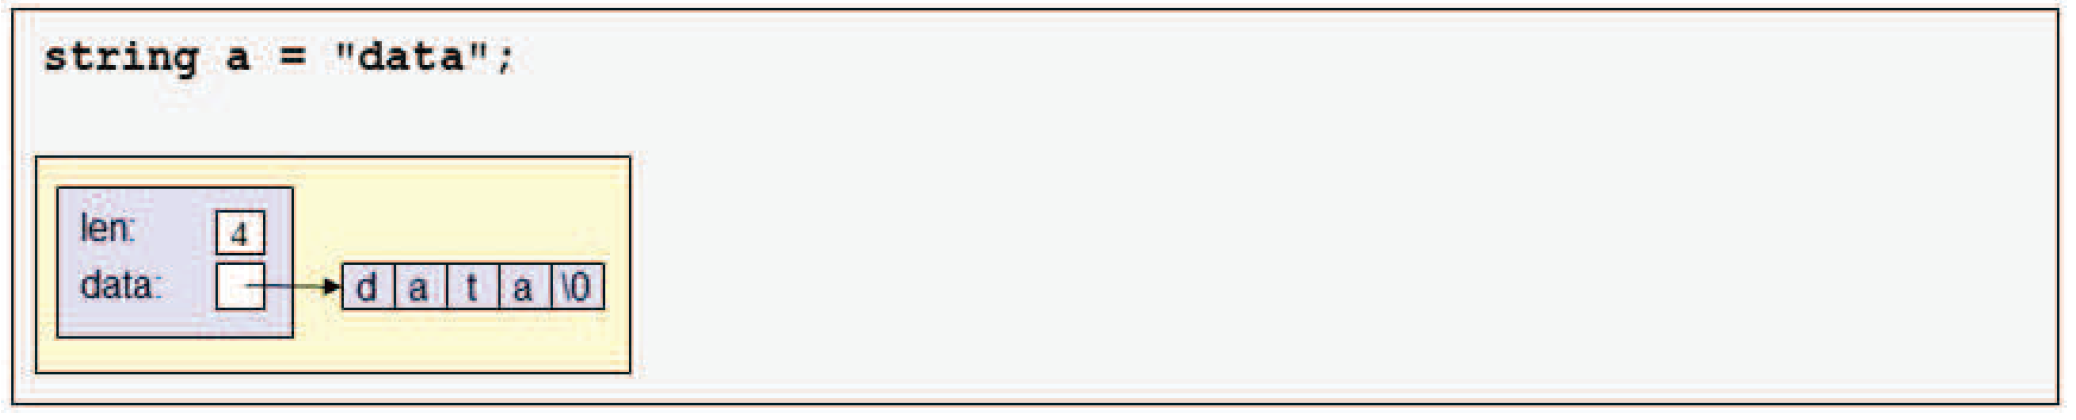
\includegraphics[width=1.0\textwidth]{content/1/chapter1/images/18}
\end{center}

上面的复制构造函数将复制成员len以获取字符数,为数据指针分配新的内存,并将源a(作为s传递)中的所有字符复制到新字符串:

\begin{center}
	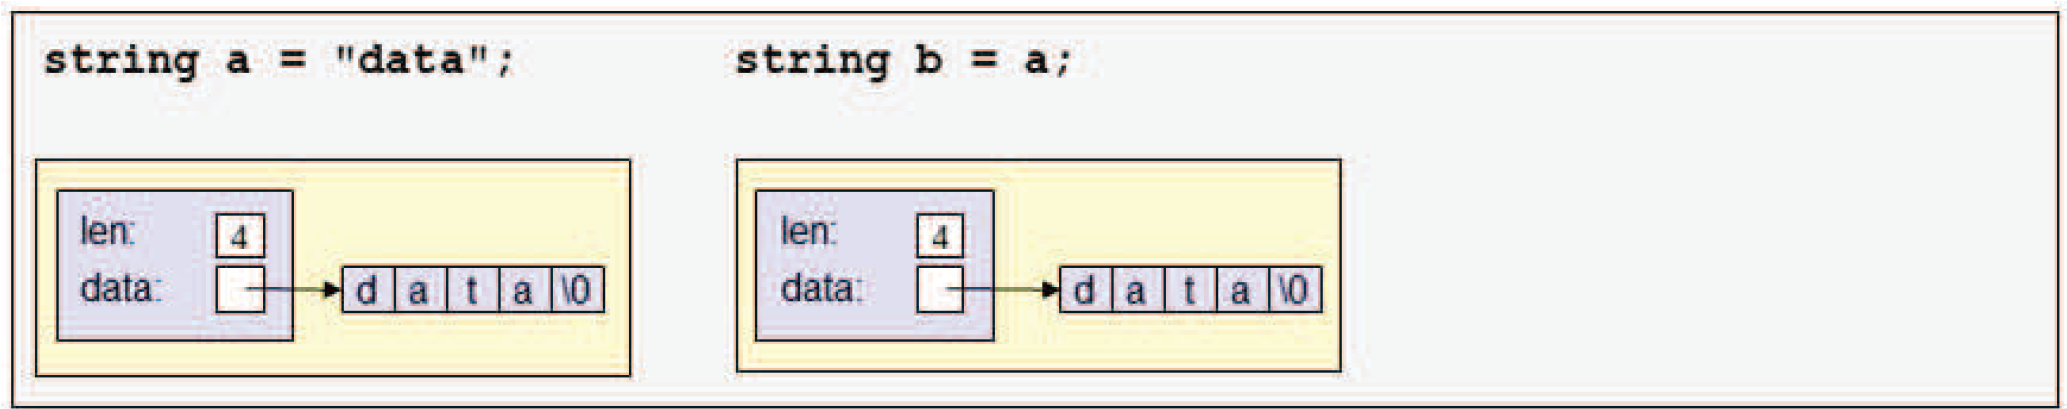
\includegraphics[width=1.0\textwidth]{content/1/chapter1/images/19}
\end{center}

\subsection{使用移动构造函数}

对于移动语义,\textit{push_back(T\&\&)}调用相应的构造函数,即\begin{cppcode}
移动构造函数
\end{cppcode}。从现有字符串创建新字符串的构造函数,和移动语义一样,构造函数使用非\textit{const}右值引用(\textit{\&\&})作为形参:

\begin{cppcode}
class string {
	private:
	int len; // current number of characters
	char* data; // dynamic array of characters
	public:
	...
	// move constructor: initialize the new string from s (stealing the value):
	string (string&& s)
	: len{s.len}, data{s.data} { // copy number of characters and pointer to memory
		s.data = nullptr; // release the memory for the source value
		s.len = 0; // and adjust number of characters accordingly
	}
	...
};
\end{cppcode}

给定上述拷贝构造函数的情况:

\begin{center}
	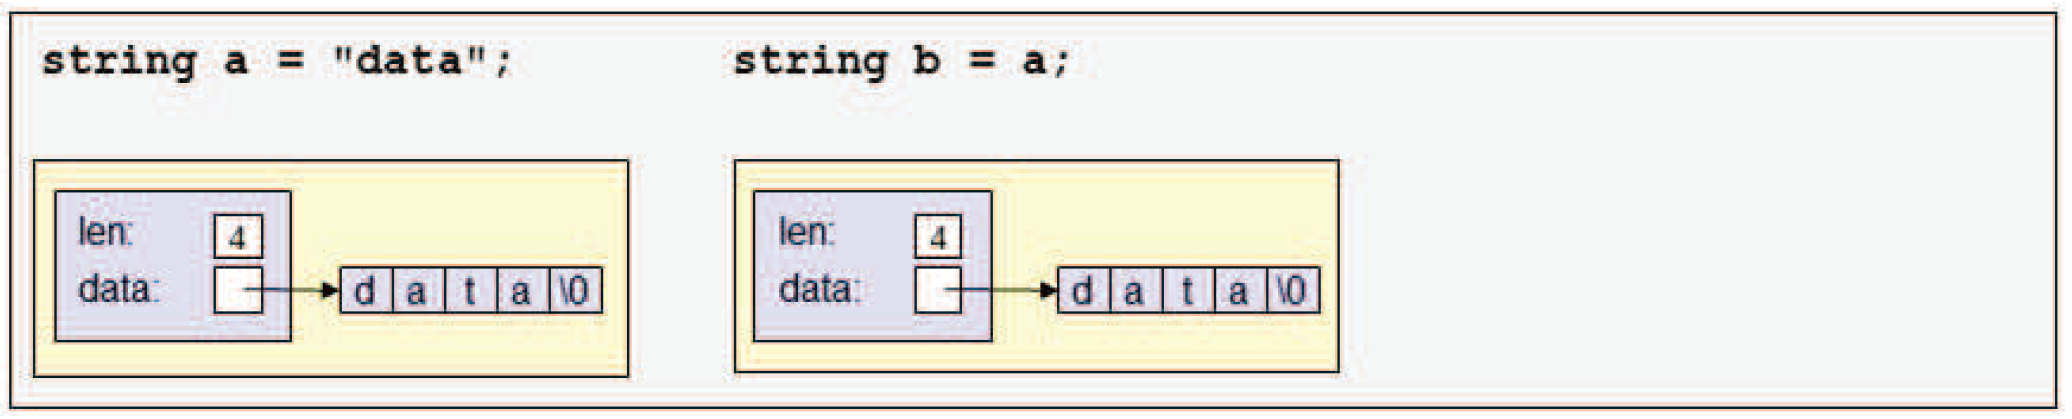
\includegraphics[width=1.0\textwidth]{content/1/chapter1/images/20}
\end{center}

我们可以这样调用string对象的构造函数:

\begin{cppcode}
std::string c = std::move(b); // init c with the value of b (no longer needing its value here)
\end{cppcode}

移动构造函数首先复制成员len和data,这意味着新字符串获得\textit{b}值的所有权(作为\textit{s}传递)。

\begin{center}
	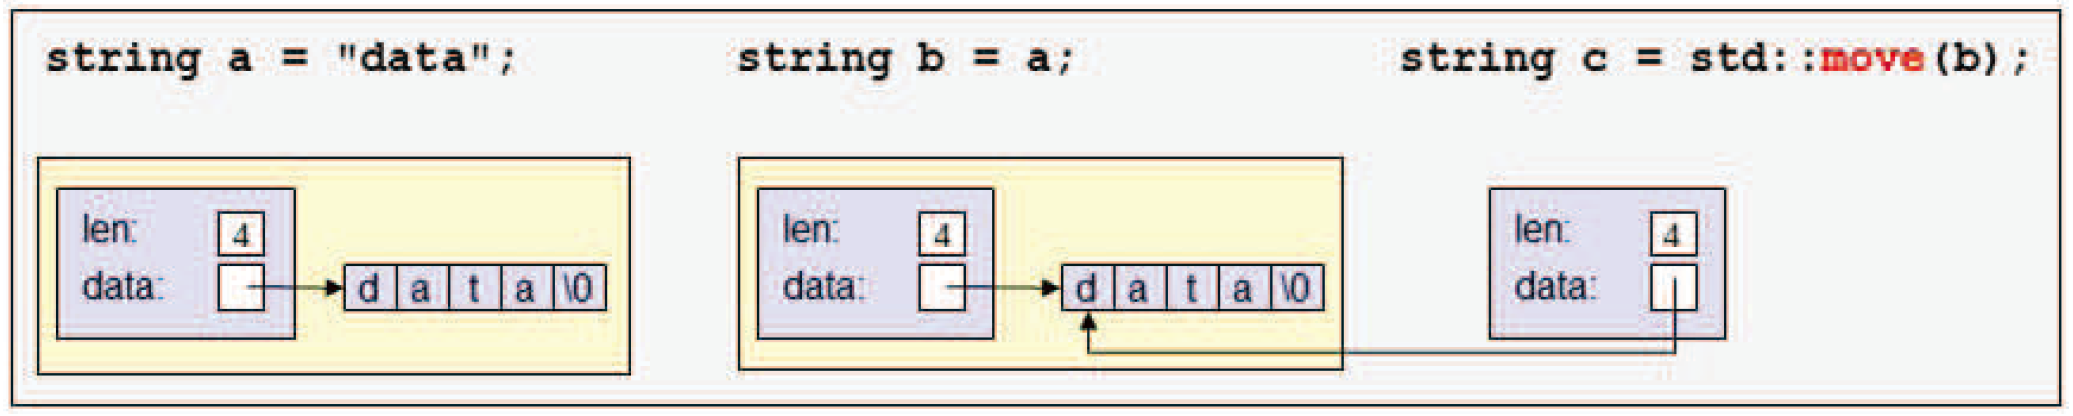
\includegraphics[width=1.0\textwidth]{content/1/chapter1/images/21}
\end{center}

这是不够的,因为\textit{b}的析构函数将释放内存。因此,我们还可以修改源字符串,使其失去内存的所有权,并使其表示空字符串:

\begin{center}
	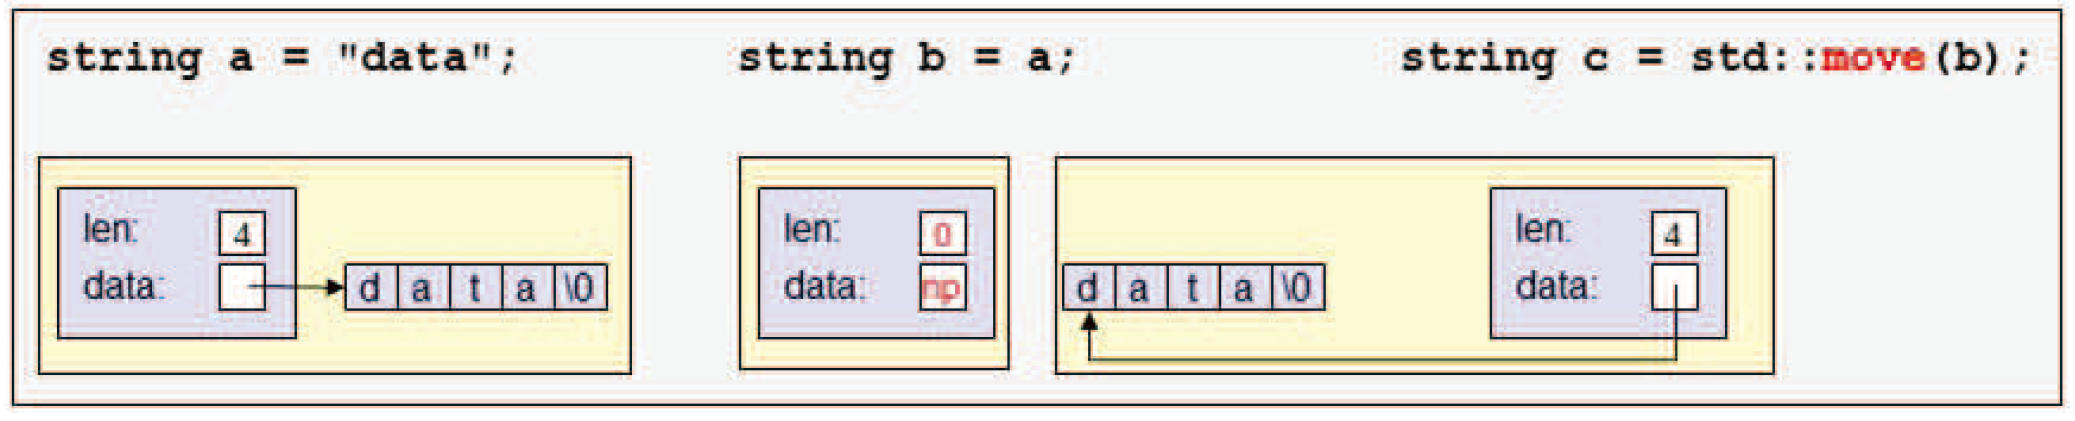
\includegraphics[width=1.0\textwidth]{content/1/chapter1/images/22}
\end{center}

结果是,\textit{c}现在有了\textit{b}的值,而且\textit{b}是空字符串。注意,唯一的保证是\textit{b}随后处于有效但未定义的状态。根据C++库中移动构造函数的实现方式,可能不为空(但通常是空的,因为这是提高性能的最简单和最好的方法)。


















